\section{Metaheuristics}\label{Solvers}
In abstract terms, our falsification procedure is based on state space search. Equipped with a representation of the search domain, which is the parameter space, the algorithm tries to make decisions to perform a sequence of moves from a given starting parameter point towards a goal parameter point that falsifies a property of interest. In words, the algorithm iteratively executes two abstract functions: (1) generate a set of candidate points and (2) test if the candidate set satisfies the falsification goal. In our falsification context, the second function entails simulating the behavior of the system associated with a given candidate parameter point and evaluating its robustness value with respect to the property. The search performance mainly depends on the first function, namely generating candidate points. 
One natural strategy for generating points is to use methods related to gradient descent, wherein new points are selected based on some estimate of the gradient of the cost function near promising, previously-evaluated points.
%One natural strategy for  generating points is focus on regions expected to yield improvement in cost, which corresponds to robustness, in our context. If no improvement is achieved, these candidates are rejected, and new candidates are generated from the current point, until no new generated candidate leads to an improvement. 
Such a descent strategy may not lead to a global optimum, leaving the search stuck around a local optimum. 
When this occurs, it is possible to restart the search from a different initial point, but this can become expensive when there are many local optima. Metaheuristics \cite{dreo:hal-01341683} are one way to go about this problem, by accepting from time to time candidates that do not improve the objective function value. In this work we combine a number of well-known metaheuristics that do not require computing gradients of the objective function. The method 
selects between two different types of search algorithms, which we describe in the following. %To distinguish them from the global combinational algorithm, we call the elementary search algorithms {\em solvers}. 

%\subsection{Exploitation-driven versus exploration-driven}

Borrowing the terminology from \cite{dreo:hal-01341683}, we {\em roughly} classify the search algorithms or solvers used in this work into two categories: 
\begin{itemize}
\item {\em Exploitation-driven} : The search algorithms in this category try to make greedy changes (often small) around the current point. We make use of a number of well-known solvers in this category, namely Simulated Annealing \cite{Kirkpatrick83optimizationby}, Global Nelder-Mead \cite{NelderMead65}, and CMA-ES (Covariance Matrix Adaptation Evolution Strategy) \cite{hansen2006eda}. This category of solvers are used to explore locally around promising points. 
%They are efficient when provided with initial points that are chosen appropriately. 
%They can be used as long as they make progresses, that is the objective values keep getting improved. 
\item {\em Exploration-driven}: The solvers of this category explore the parameter space widely, and thus quickly enlarge the exploration space. Such solvers are particularly useful to help the exploration escape local optima, where the objective value has stagnated. The exploration-driven solver we use in this work is a pseudo-random sampling method. Note that the pseudo-random search method does not need an initial point, as shown in Algorithm \ref{algoSolverCombination}. 
\end{itemize}
The above classification refers only to behaviors of the solvers seen on a global level, since the above-mentioned metaheuristics can contain both exploitation-driven and exploration-driven aspects. Consider the basic idea behind each of the solvers that we classify as exploitation-driven. 
The Simulated Annealing metaheuristic \cite{Kirkpatrick83optimizationby} was inspired by the annealing technique in metallurgy to attain solid state with low energy. The algorithm makes a modification to the current point and if this modification decreases the objective function $E$ (which is energy in the annealing process), it is accepted; otherwise it is accepted with a probability $e^{\frac{-\delta E}{T}}$, where $\delta E>0$ is the difference between in the objective function value of the new point and the current value. The temperature $T$, used to control the process, is first set at a high value for a number of iterations, which facilitates exploration, since new points are often accepted.
%a good chance of reaching a region with potential of containing a global optimum. 
Then the temperature is lowered to facilitate exploitation within this region. For the Nelder-Mead algorithm \cite{NelderMead65}, a simplex is iteratively transformed over which the objective function is extrapolated. It replaces the worst vertex of a simplex by a point symmetric to it with respect to its opposing face. If the vertex point is better, then the simplex is stretched along this line; otherwise it is contracted toward the best vertex. This algorithm is exploitation-driven, though a globalized version includes probabilistic restarts \cite{CHANG2012684}. Regarding the CMA-ES algorithm \cite{hansen2006eda}, a population of new candidate points is generated according to a multi-variate normal distribution. For each generation, the mean value of the distribution is updated using recombination and selection mechanisms of the Evolution Strategy. The update of the covariance matrix is similar to a descent in the direction of a sampled natural gradient of the expected objective function value. In the CMA-ES algorithm, the exploration feature lies in the recombination; however, in general this algorithm is more exploitation-driven. A variant of the algorithm with restarts dynamically increases the population size \cite{hansen2006eda}. Each of Simulated Annealing, Global Nelder-Mead, and CMA-ES possesses qualities of exploration and exploitation, but we consider them here as exploitation methods, since the core search strategy for each involves remaining within a region near the current best solution.

The exploitation methods make effective use of local information regarding the shape of the cost surface, but they can become stuck near local optima. Exploration methods avoid this problem, but they do make effective use of local information. To achieve an effective method that combines exploitation and exploration techniques, it is important to have appropriate measures for exploitation and exploration performance. Exploitation performance can be measured by the reduction of the robustness value. Exploration performance can be measured using the notion of coverage. In the optimization process, we use a signal value coverage measure instead of timed pattern coverage, because the timed pattern generation is guaranteed to have good coverage. Before describing how we use these measures to guide our metaheuristics combination approach, we briefly recall the signal value coverage notion.

\paragraph{Signal value coverage as exploration performance measure}	

The signal value coverage is defined using a metric called {\em cell occupancy}. Note that our set of signals takes values in the set $\inputparamset$.
Let $\omega=\{ \omega_i | i=1,\ldots,
\numpartition \}$ be a partition of $\inputparamset$. For now, we assume that each partition element,
which we call a \emph{cell}, is rectangular, with each side of equal
length, $\Delta$, called \emph{grid cell size}. A
vector that indicates how many points are in each cell is called a
\emph{distribution}, $\distribution=(k_1,\ldots, k_\numpartition)$,
where each $k_i$ indicates how many points are located in cell $i$.
Cell occupancy is based on the relative number of cells occupied by
points, compared to the total number of cells. Consider the total
number of occupied cells, that is, the number of cells that contain
at least one point, i.e., $\occupiedcellcount =  \sum_{i=1}^{\numpartition} c_i$  
where $c_i = 1$ if  $k_i\geq 1$, and $c_i = 0$ otherwise. Then, the proposed cell occupancy measure is given as
$\celloccupancy(\distribution) = \displaystyle{ \frac{\log \occupiedcellcount}{\log \numpartition}}$.
Logarithm functions are used due to the fact that the total number of cells could be very large as compared to the number of occupied cells. The logarithms provide two key features for the cell occupancy measure: (1) they maintain the monotonicity of the measure, and (2) they result in reasonable measure values even for cases where the dimension $\cpdim$ is  large. 
%This difficulty is illustrated for the Simulated Annealing and Nelder-Mead algorithms in Figure \ref{fig:solverproblems}. 
%\begin{figure}
%%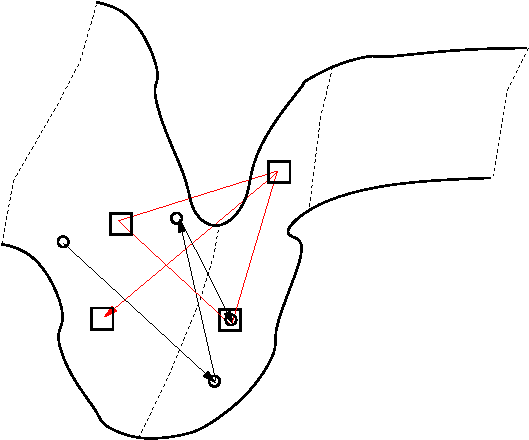
\includegraphics[scale=0.3]{LocalOptima.pdf_t}
%\input{LocalOptima.pdf_t} 
%\caption{Illustration of a situation where the search gets stuck around a local minimum at the bottom of a ``valley'' surface representing the cost $\rho$ as function of a two-dimensional parameter. The sequence of circles ($p_1, p_2, p_3, p_4$) represents the sequence of points generated using Simulated Annealing. Then the Nelder-Mead algorithm is used from $p_4$ and it produces first the triangle (the vertices of which are drawn with squares)  $\{p_4, p_5, p_6 \}$ and then creates a new vertex $p_7$ by reflection of $p_5$ with highest cost value. It can be seen that even by switching between these two solvers, it is not possible to escape the ``valley'' around this local minimum, and an exploration-driven search is needed.} \label{fig:solverproblems}
%\end{figure}

\section{Guided combination of metaheuristics} \label{sec:combination}
In this section, we describe our algorithm for guided combination of metaheuristics. Before continuing, we remark that a solver is often configurable, that is, its configuration parameters can be modified. For example, consider the Simulated Annealing solver: the configuration parameters include the initial temperature, the number of iterations in one temperature stage, and the temperature cooling rate. Indeed, a number of approaches to learning these configuration parameters have been proposed in the literature (see for example \cite{HutHooLey11-smac} and references therein). %For simplicity of presentation, we omit the internal configurations of the solvers. \textcolor{red}{However, a method for selecting promising initial points for the next explorations can be applied to automatically tune solver configurations. <- What is the point? Are we doing this or do we have a reference? If no, then maybe omit?}

%\begin{algorithm}
%\caption{Search-based Falsification}
%\begin{algorithmic}
%%\Require  
%%\Ensure  		
%	        %\State $\solver = Select(\overline{\solverset})$
% 		%\State $\overline{\solverset} = \overline{\solverset} \setminus \solver$
%		%\State
%		\ForAll{$\solver \in \solversetall$} 
%		\State $\neighstateSet = NeighborGeneration(\state)$
%		\State \Comment{{\sf run solver $\solver$ for $\exectime_{\solver}$ time from initial points $\Gamma$}}
%  		\State $\{ \bestobj, \explostateSet \} = Run(\solver, \Gamma, \exectime_{\solver})$ 
%		\EndFor
%\end{algorithmic}
%\end{algorithm}


\begin{algorithm}
\caption{Abstract algorithm for combining metaheuristics \label{algoSolverCombination}}
\begin{algorithmic}
%\Require  
%\Ensure  
\State \Comment{{\sf $\solver$ is the solver index}}
\State \Comment{{\sf $\solversetRho$ is set of exploitation-driven solvers}}
\State \Comment{{\sf $\explostateSet$ is set of visited states}}
%\State \Comment{$\explostateSet = (\explostateSet_{\solver})_{\solver \in \solversetall}$ is vector of all $\explostateSet_{\solver}$}
\State \Comment{{\sf  $k_{max}$ is the maximal number of iterations}}
\State

\State $k= 1$
%\State $blocking = false$
%\State $\forall \solver  \in  \solversetall, \explostateSet_{\solver} = \emptyset$   	
\While{$k \le k_{max}$}  
      %\State \Comment{{\sf  $\solverset$ is the set of all available exploitation-driven solvers}}
       %\State $\overline{\solverset}= \solverset$    \Comment{{\sf  $\overline{\solverset}$ is the set of solvers to run in this round}}
      % \State $\explostateSet_o = \explostateSet$  \Comment{{\sf Store the previous set of visited states in $\paramset_o$}}
	        %\State $\solver = Select(\overline{\solverset})$
 		%\State $\overline{\solverset} = \overline{\solverset} \setminus \solver$
		%\State		
		\State \Comment{{\sf executing all the exploitation-driven solver $\solver$}}
  		\State $\{ \bestobj, \explostateSet \} = Exploitation(\solversetRho, \explostateSet)$ 	 
	 
         \State
\State $\coverage = updateCoverage(\coverage,  \explostateSet)$
\State
\State \Comment{{\sf blocking detection based on coverage and robustness evolution}}
\State $blocking =  DetectBlocking(\coverage, \bestobj)$ 
 \If{($blocking$)}
	 \State $\solver = PseudoRand$
	 \State \Comment{{\sf run the pseudo-random solver for $\exectime_{\solver}$ time}}   
	 \State $(\bestobj, \explostateSet)= Run(\solver, \exectime_{\solver})$ 
 \EndIf	
 \State        
\State $k++$
\EndWhile
\end{algorithmic}
\end{algorithm}

Our method is essentially is organized in iterations, as shown in Algorithm \ref{algoSolverCombination}, and in each iteration the solvers are called based on the current search results. First, the number of iterations $k$ is initialized to $1$. Then, a loop begins iterations of the search procedure, starting with $Exploitation$, which adds to the set of visited states $G$ by running each of the exploitation-based solvers in the set $\solversetRho$ (the letter $\rho$ indicates that these solvers are used to improve the robustness). Based on the updated list of visited points, $updateCoverage$ computes a value $H_c$ that captures the degree to which the parameter space is covered by the points in $G$.  Next, the procedure $DetectBlocking$ determines whether the cost value $\rho$ has stagnated. If it has, then the $blocking$ flag is set and the exploration-based $PseudoRand$ search procedure is run for $T_s$ seconds. If blocking is cleared, then the next iteration of the procedure begins. Below, we describe aspects of Algorithm \ref{algoSolverCombination} in more detail.

\paragraph{Exploitation to improve robustness.}

We describe the $Exploitation$ procedure that appears in Algorithm \ref{algoSolverCombination} and is shown in detail in Algorithm \ref{algoSolverExpl}. 
%We specify a maximum computation time budget $T_s$ for each exploitation-based solver. 
%because arriving at a global optimum is not feasible from all possible parameter points. 
%We denote the set of exploitation-driven solvers by $\solversetRho$ (the letter $\rho$ indicates that these solvers are used to improve the robustness). 
An exploitation-driven solver with index $\solver$ starts from a set $\Gamma$ of initial points for execution time $\exectime_{\solver}$. The corresponding best cost value is denoted by $\bestobj$. Throughout the search process, we maintain a set $\explostateSet$ of {\em intermediate visited states}, which is initially empty. By {\em visited state}, we mean the pair $(\param, \bestobj)$ where $\param$ is a parameter point and $\bestobj$ is its associated cost values, and by `intermediate' we mean the points successively computed by the solver scheme. The reason we store the visited states is that they can reflect the relation between the cost function and the parameter and can thus indicate promising regions for subsequent iterations. Note that in this abstract algorithm, the states in $\explostateSet$ are not distinguished by the solvers that generate them; however, in our implementation, we store states visited by each solver $\solver$ separately, because we want to avoid applying a solver to a point explored previously by the same solver, unless it is the last visited point. Indeed, some solvers are not stochastic; therefore, under the same configuration and from the same initial point, such solvers follow the same path. We use the intermediate visited states to derive good initializations for subsequent solvers, which is captured by the function $InitialPointSelection(\explostateSet)$ in Algorithm \ref{algoSolverExpl}. We discuss this in more detail below.

\begin{algorithm}
\caption{$\{ \bestobj, \explostateSet \}=Exploitation(\solversetRho, \explostateSet)$ 
(Executing the exploitation-driven solvers) \label{algoSolverExpl}}
\begin{algorithmic}
%\Require  
%\Ensure  		
	        %\State $\solver = Select(\overline{\solverset})$
 		%\State $\overline{\solverset} = \overline{\solverset} \setminus \solver$
		%\State
		\State \Comment{{\sf $\exectime_{\solver}$ is max time for each solver}}
		\ForAll{$\solver \in \solversetRho$} 
		\State $\Gamma = InitialPointSelection(\explostateSet)$
		\State \Comment{{\sf run solver $\solver$ for $\exectime_{\solver}$ time from initial points $\Gamma$}}
  		\State $\{ \bestobj, \explostateSet \} = Run(\solver, \Gamma, \exectime_{\solver})$ 
		\EndFor
\end{algorithmic}
\end{algorithm}


%On the other hand, one need not start uniquely from the best points that have been found so far, the previous explorartion states can indicate promising regions to the next solvers. For example, if the next solver is CMA-ES (the principle of which is to update the mean and the covariance matrix of normally distributed samples in each of its internal iteration), we can define an initial mean and a covariance matrix using only the previously explored points with good objective values. We defer a discussion on this initialization procedure for each solver in Section \ref{sec:init}. 

\paragraph{Exploration to escape local minima.}
We now describe a situation where an exploitation-driven solver is stuck around a local optimum. It is important to be able to detect such blocking situations in order not to waste computation effort further. One possible next step is to switch to another solver, since different solvers using different search methods may take the current search out of the local optima. The search is said to be {\em blocking}, if it does not improve the cost value within some execution time limit using any available exploitation-driven solver. Recall that in our falsification context, cost functions are robustness functions of output trajectories of the dynamical system in \ref{eq:behaviorfunc}. Once a blocking state is detected, an exploration-driven solver, such as a pseudo-random search method, can be used to escape that blocking state. 

To detect a blocking situation, we monitor the coverage and robustness evolution. More concretely, when both the robustness and coverage values remain stagnant, that is, they do not decrease and increase respectively by some predefined amounts, for a predefined number of iterations, we consider the search to be in a blocking situation. Due to the monotonicity of the coverage and robustness evolution with respect to the number of visited parameter points, the detection of a blocking state can be performed by comparing the coverage and the robustness values of the current iteration and those of the previous iteration. This process is captured by the function $DetectBlocking$ in Algorithm \ref{algoSolverCombination}.

\paragraph{Solver Initialization.}\label{sec:init}
We describe the $InitialPointSelection$ function in Algorithm \ref{algoSolverExpl}, which selects initial parameter points for a solver. We propose three heuristics to do so:
\begin{itemize}
\item The first heuristic is to select an initial point or a population of initial points from the best points obtained from previous iterations, and repeat this process until achieving a satisfying result. Although different solvers are used, such a greedy method can still lead to a blocking state. 
\item Using an exploration-based approach, we can uniformly sample points over the parameter space, which is essentially what the above-mentioned pseudorandom sampling method does. This, however, does not allow an iteration to exploit the results of the previous iterations. 
\item The third heuristic is to pick initial parameter points according to a distribution that is dynamically updated based on the previous results. This idea, inspired by the population based methods such as the CMA-ES, is described in the sequel. 
\end{itemize}

\paragraph{Iteratively updated initial point sampling distribution.}
As described above, after each iteration we keep the points visited in the previous iterations. In each iteration we select a set $\mathcal{B}$ of best points, the robustness values of which are below some threshold, and use them to define the sampling distribution for new candidates. 
%The iterative sampling process can be summarized by three steps in the $k^{th}$ iteration: 
%\begin{itemize}
%\item sample $N^k$ candidates based on a probability model; 
%\item evaluate the sampled candidates; 
%\item update the probability model for the sampling process in the next round.
%\end{itemize}
Let $\param \in \real^n$ be a parameter point, let $\param_i$ denote its $i^{th}$ coordinate. For any point $\param$ in $\mathcal{B}$, let $[\underline{\param}_i, \overline{\param}_i]$  be the bounding interval such that each coordinate $\param_i \in [\underline{\param}_i, \overline{\param}_i]$. In the $k^{th}$ iteration, the sampling distribution of $\param_i$ can be a normal distribution $\mathcal{N}(\overline{\param}^k_i, \sigma_i^k)$, where the mean $\overline{\param}^k_i$ is one of the most promising candidates from the previous iteration, selected based on the robustness value. The standard deviation $\sigma_i^k$ in the $k^{th}$ iteration can be determined by: 
\begin{equation} \label{eq:sigma}
\sigma_i^k = (\overline{\param}_i - \underline{\param}_i) (\frac{1}{N^k})^{k/n}
\end{equation}
which decreases iteration after iteration. The number $N^k$ of candidates can vary, being large at the beginning and decreasing gradually. In the first iteration where no information is available, we can sample candidate parameter points according to a uniform distribution. 


\paragraph{Keeping promising points.}
Running a solver from the points visited by the other solvers can make the set of visited states quickly become large. Thus, we keep only {\em promising} points. Note that a promising point is not necessarily among the best points. It is simply a point that is still worth being kept. To this end, we will make use of a well-known method for tuning algorithm configurations, called F-Race \cite{Birattari2010}, which was inspired from racing algorithms in machine learning. F-Race is used to evaluate a given set of algorithm configurations iteratively on a sequence of problem instances. When there is sufficient statistical indication that a configuration performs poorly, it is excluded from the future search process. In our falsification setting, we will use these concepts with slightly different meanings. Indeed, we have only one problem instance (defined by a dynamical system and a property), but a number of available solvers; however, we follow the spirit of the algorithm configuration tuning approach, by letting solver initial points play the role of algorithm configurations.

%Let $c(\param, \solver)$ be a variable representing the cost function value obtained by running the solver $\solver$ from the point $\param \in \paramset$. Note that $c(\param, \solver)$ can be thought of as a random variable because of the randomized elements in some solvers. 

%We describe how the F-Race algorithm is integrated into the exploitation procedure to remove from consideration the visited points that are not promising. In the first iteration, no visited points are available, we randomly sample a set of parameter points $\Gamma^0$, which serve as initial candidates. Then, to each candidate, we apply the available solvers for some time and record the corresponding costs. The statistical information from the recorded costs is used to decide if a parameter point is not promising at all and thus is dropped. Suppose again that the current iteration is $k$ and let $\Gamma^k$ be the set of the candidates that are still in the race. Let $m_k = | \Gamma^k | $ be the size of the set $\Gamma^k$. Let $m_s$ be the number of solvers, that is $m_s = | \solversetall|$. The Friedman test assumes that the costs are $m_k$ mutually independent $m_s$-variate random variables. For each solver $\solver$, we construct a cost vector $C^k_s$ which is of size at most $m_k$
%\begin{eqnarray}\label{eq:C}
%C^k_s = (c_{\solver}(\param^{q_1}), c_{\solver}(\param^{q_2}), \ldots, c_{\solver}(\param^{q_{m_k})})
%\end{eqnarray}
%Each element of the vector is defined by $c_{\solver}(\param^{q_i}) = c(\param^{q_i}, \solver)$ and corresponds to the best cost obtained by executing the solver $\solver$ from the point $\param^{q_i}$ after a completed run. If a parameter point has not been used with a solver $\solver$, it is not included in the cost vector for the Friedman test but is kept for consideration. The costs $c_{\solver}(\param^{q_i})$ are ranked in non-decreasing order, that is $q_i \le q_{i'}$ if $c_{\solver}(\param^{q_i}) \le c_{\solver}(\param^{q_{i'}})$. For each parameter point $\param^{q_i}$, let $R^{\solver}_{i}$ be the rank of $\param^{q_i}$ with respect to the solver $\solver$. Let $R_{i} =  \sum_{\solver=1}^{m_s} R^{\solver}_{i}$ be the sum of ranks for $\param^i$ ($1 \leq i \leq m_k$) over all the solvers. To perform the Friedman test \cite{GVK24551600X}, we determine
%\begin{eqnarray*}
%\displaystyle \tau & = \displaystyle{ \frac{ (m_k-1) \sum_{i=1}^{m_k} (R_i - (\frac{m_s(m_k+1)}{2})^2 } {\sum_{s=1}^{m_s} \sum_{i=1}^{m_k}  (R^s_{i})^2 -  \frac{m_s m_k (m_k+1)^2}{4} }}  \nonumber \\ 
%\end{eqnarray*}
%If the value of $\tau$ is larger than the $(1 - \alpha)$ quantile of the distribution $\chi^2$  with $(m_k - 1)$ degrees of freedom ($\alpha$ is a predefined value), the null hypothesis that all parameter values are equivalent is rejected \cite{AP91}. If at the $k^{th}$ iteration this hypothesis is not rejected, we keep the current set of parameter points. If the null hypothesis is rejected, the candidates with the lowest expected rank are considered the most promising parameter values. We then remove, from the current set, the points with differences in cost beyond some given threshold.  
 %(average ranks are used in case of ties)
 
%All the above-described developments are summarized in Algorithm \lref{algoFRace}), which uses the heuristic using updated initial point sampling distributions and the F-Race method to retain promising points. This represents one heuristic, though we note that the two first heuristics for initial point selection can also be used in place of this method.
%
% 
%\begin{algorithm}
%\caption{Exploitation in the $k^{th}$ iteration of \ref{algoSolverCombination}}
%\caption{$\{ \bestobj, \explostateSet \}=Exploitation(\solversetall, \explostateSet, k)$ \label{algoFRace}}
%\begin{algorithmic}
%%\Require  
%%\Ensure  
%%\State $k = 1$
%%\State $\Gamma^{k-1}=\emptyset$
%%\While{$k \le k_{max}$} 
%  \State \Comment{{\em Sample new $N^k$ parameter values using distribution $\pi^k$}}
%  \State
%  \State $\Gamma  = Sample(\explostateSet, N^{r}, \pi^r)$
%   \State
%  \ForAll{$\solver \in \solversetRho$} 
%   % \State $\Gamma = InitialPointSelection(\explostateSet)$
%    \State
%     \State \Comment{{\em Run solver $\solver$ from some parameter points in $\Gamma$, if it is not done, for $\exectime_{s}$ time}}    
%    % \State \Comment{{\em Some intermediate explored points are added in $\Gamma^k$ to produce the new set  $\Gamma^k$} }   
%      \State $\{ \bestobj, \explostateSet \} = Run(\solver, \Gamma, \exectime_{\solver})$   
%      \State 
%      \State  Update the cost vector $C_s^k$ for these parameter points and their costs in $\explostateSet$ as in (\ref{eq:C})
%     %\State $C^k =  C^k \cup c(\Theta^k, A_s, t_{s}^k)$  
%     \EndFor
%   \State
%   \State Run F-Race based algorithm on the cost vectors to exclude the least promising candidates from $\explostateSet$   
%   \State
%  %\State $k++$  %\Comment{{\em Increment the iteration counter}} 
%  \State Update distribution $\pi_i^k=\mathcal{N}(\overline{\param}^k_i, \sigma_i^k)$ for each $i^{th}$ parameter coordinate, using the mean $\overline{\param}^k_i$ and the deviation $\sigma^k_i$ as in (\ref{eq:sigma})
%%\If{}
%%\ElsIf{ }
%%\EndIf
%%\EndWhile
%\end{algorithmic}
%\end{algorithm}
